\documentclass[pdflatex,sn-mathphys-num]{sn-jnl}

\usepackage{graphicx}
\usepackage{multirow}
\usepackage{amsmath,amssymb,amsfonts}
\usepackage{amsthm}
\usepackage{mathrsfs}
\usepackage[title]{appendix}
\usepackage{xcolor}
\usepackage{textcomp}
\usepackage{manyfoot}
\usepackage{booktabs}
\usepackage{algorithm}
\usepackage{algorithmicx}
\usepackage{algpseudocode}
\usepackage{listings}

\raggedbottom

\begin{document}

\title[Perfil estacional global para el pronóstico de ventas minoristas]{Pronóstico mensual de ventas minoristas por categoría y región con un perfil estacional global sobre un índice libre de escala: un modelo de doce parámetros frente a Random Forest, XGBoost y otros siete métodos en Sample Superstore}

\author[1]{\fnm{Alex} \sur{Teran}}

\author[1]{\fnm{David} \sur{Estrada}}

\affil[1]{\orgname{Universidad del Norte}, \orgaddress{\city{Barranquilla}, \country{Colombia}}}

\abstract{La planificación comercial de una cadena minorista requiere pronósticos mensuales de ventas por categoría y región, pero a ese nivel las series son cortas, ruidosas y de escalas distintas. Este trabajo formula el problema como una regresión supervisada sobre el conjunto público Sample Superstore (9{,}994 líneas de pedido, 2014--2017), agregado en un panel de 12 series y 48 meses, y propone un perfil estacional global contraído: un modelo de doce parámetros que predice un índice de ventas libre de escala (ventas del mes divididas por el promedio de los doce meses previos) combinando el patrón estacional común a todas las series con el rezago anual de cada una. Se comparó con el pronóstico ingenuo estacional y con ocho regresores (Ridge, Lasso, regresión bayesiana, KNN, árbol de decisión, Random Forest, XGBoost y SVR) en una evaluación de origen móvil con 24 orígenes mensuales, en la que todos los modelos se reentrenan y reajustan sus hiperparámetros con validación cruzada temporal anidada. El modelo propuesto obtuvo el menor MAE, 2{,}307 $\pm$ 846 USD por serie y mes, frente a 2{,}366 de SVR, 2{,}423 de Random Forest y 2{,}728 del ingenuo estacional, y el menor tiempo de ajuste (0.45 ms, doce veces menos que el modelo entrenado más rápido y unas 760 veces menos que Random Forest). Tras la corrección de Holm, la prueba de Diebold--Mariano respalda la diferencia frente al ingenuo estacional y XGBoost; frente a las demás referencias la ventaja no es estadísticamente concluyente. La ablación indica que agrupar las series es el componente decisivo y que el nivel móvil evita un sesgo de $-25$\% en el total.}

\keywords{Pronóstico de ventas minoristas, Regresión supervisada, Perfil estacional global, Índice libre de escala, Error absoluto medio, Prueba de Diebold--Mariano}

\maketitle

\section{Introducción}\label{sec:intro}

Pronosticar las ventas es un insumo directo de la planificación minorista: de la cifra esperada dependen las metas de cada región, las compras de inventario de cada categoría y el presupuesto de ingresos del año siguiente \cite{fildes2022}. Esas decisiones no se toman sobre el total de la empresa sino sobre combinaciones de producto y territorio, y a ese nivel de desagregación las series son más cortas, más ruidosas y de tamaños muy distintos entre sí, lo que dificulta tanto el ajuste de un modelo como la comparación honesta entre varios \cite{fildes2022,hyndman2021}.

La práctica habitual en empresas pequeñas y medianas es proyectar ``lo mismo que el mismo mes del año anterior''. Este pronóstico ingenuo estacional captura la estacionalidad sin estimar ningún parámetro y es la referencia mínima que cualquier método debe superar \cite{hyndman2021}, pero arrastra el nivel de hace doce meses y el ruido de un único mes: cuando la empresa crece, subestima de forma sistemática. Los modelos de aprendizaje automático ofrecen una alternativa. Las competencias recientes de pronóstico, en particular M5 con ventas minoristas jerárquicas, mostraron que los ensambles de árboles entrenados sobre muchas series a la vez dominan a los métodos que ajustan cada serie por separado \cite{makridakis2022}, y la teoría de los modelos globales explica por qué: compartir parámetros entre series aumenta el tamaño efectivo de la muestra \cite{monteromanso2021}.

Tres limitaciones impiden trasladar esos resultados a un panel pequeño. Primera, los ensambles como Random Forest \cite{breiman2001} y XGBoost \cite{chen2016} tienen cientos de árboles y varios hiperparámetros; con unas pocas centenas de observaciones su flexibilidad se gasta en ajustar ruido, y su costo de entrenamiento es órdenes de magnitud mayor que el de un modelo simple. Segunda, un modelo global necesita series comparables; las soluciones más exitosas normalizan cada serie por su nivel \cite{salinas2020,smyl2020}, y los árboles, además, no extrapolan fuera del rango visto en entrenamiento. Tercera, con pocos meses de evaluación las diferencias entre modelos suelen ser menores que su variabilidad, y una tabla de errores promedio sin pruebas de capacidad predictiva \cite{diebold1995,giacomini2006} ni corrección por comparaciones múltiples \cite{holm1979} puede atribuir al modelo lo que es azar de la partición \cite{cerqueira2020}.

Este trabajo aborda el problema sobre el conjunto público Sample Superstore \cite{superstore}, que registra las ventas de una cadena minorista de Estados Unidos entre 2014 y 2017 en tres categorías de producto y cuatro regiones. Una primera versión del estudio seleccionó un Random Forest global por validación cruzada; el análisis de ese modelo mostró que su señal provenía casi exclusivamente del mes del año y del rezago anual. De esa observación nace la propuesta: estimar directamente lo que el ensamble aprendía de forma indirecta. Las contribuciones son tres. (i) Se formula el pronóstico mensual por categoría y región como una regresión sobre un \emph{índice de ventas libre de escala}, las ventas del mes divididas por el promedio de los doce meses anteriores de la misma serie. (ii) Se propone un \emph{perfil estacional global contraído}: doce parámetros, uno por mes del año, estimados con las doce series agrupadas y combinados con el rezago anual de cada serie mediante un peso elegido por validación cruzada; el ingenuo estacional es un caso particular del modelo. (iii) El modelo se compara con el ingenuo estacional y con ocho regresores (Ridge \cite{hoerl1970}, Lasso \cite{tibshirani1996}, regresión bayesiana \cite{mackay1992}, KNN \cite{cover1967}, árbol de decisión \cite{breiman1984}, Random Forest \cite{breiman2001}, XGBoost \cite{chen2016} y SVR \cite{drucker1997}) en una evaluación de origen móvil con reentrenamiento y reajuste mensual, sometida a pruebas de Diebold--Mariano, Giacomini--White y bayesiana con región de equivalencia práctica, tamaños de efecto, ablación por componente, sensibilidad y costo computacional.

La hipótesis de trabajo es que el perfil estacional global supera al ingenuo estacional y a los ocho regresores en error absoluto medio y en tiempo de cómputo. En la evaluación de origen móvil el modelo propuesto obtiene el menor error de los diez métodos, 15.4\% por debajo del ingenuo estacional, 4.8\% por debajo de Random Forest y 2.5\% por debajo de SVR, y el menor tiempo de ajuste e inferencia entre los modelos entrenados. La evidencia estadística es concluyente frente a dos de las nueve referencias y favorable, pero no concluyente, frente a las demás; así se reporta.

\section{Metodología}\label{sec:metodologia}

\subsection{Formulación del problema y notación}\label{subsec:formulacion}

Sea $y_{s,t}\ge 0$ la venta en dólares (USD) de la serie $s\in\{1,\dots,S\}$, una combinación de categoría y región, en el mes $t\in\{1,\dots,T\}$, con $S=12$ y $T=48$. Se define el nivel reciente de la serie y su índice de ventas como
\begin{equation}
\ell_{s,t}=\frac{1}{12}\sum_{j=1}^{12}y_{s,t-j},\qquad z_{s,t}=\frac{y_{s,t}}{\ell_{s,t}},
\label{eq:indice}
\end{equation}
de modo que $z_{s,t}=1.3$ significa vender 30\% más que el promedio de los doce meses previos. La tarea es aprender una función $f:\mathcal{X}\to\mathcal{Y}$, con $\mathcal{Y}=\mathbb{R}_{\ge 0}$, que prediga el índice a partir de un vector $\mathbf{x}_{s,t}\in\mathcal{X}$ construido únicamente con información disponible antes de iniciar el mes $t$:
\begin{equation}
\mathbf{x}_{s,t}=\Bigl(c_s,\;r_s,\;\tfrac{y_{s,t-12}}{\ell_{s,t}},\;\tfrac{y_{s,t-1}}{\ell_{s,t}},\;\tfrac{1}{3\ell_{s,t}}\textstyle\sum_{j=1}^{3}y_{s,t-j},\;\sin\tfrac{2\pi m_t}{12},\;\cos\tfrac{2\pi m_t}{12}\Bigr),
\label{eq:x}
\end{equation}
donde $c_s$ y $r_s$ son la categoría y la región de la serie y $m_t\in\{1,\dots,12\}$ el mes del año. Los modelos de referencia usan el vector completo; el modelo propuesto solo necesita $m_t$ y el rezago anual relativo $r^{(12)}_{s,t}=y_{s,t-12}/\ell_{s,t}$. El pronóstico en dólares se recupera con
\begin{equation}
\hat{y}_{s,t}=\max\bigl(0,\;\hat{f}(\mathbf{x}_{s,t})\,\ell_{s,t}\bigr).
\label{eq:retorno}
\end{equation}
El criterio de selección de modelos e hiperparámetros es el error absoluto medio sobre el índice,
\begin{equation}
\mathcal{L}_{\mathrm{MAE}}=\frac{1}{n}\sum_{i=1}^{n}\bigl|z_i-\hat{z}_i\bigr|,
\label{eq:perdida}
\end{equation}
elegido por su robustez ante los valores atípicos que revela el análisis exploratorio; cada algoritmo conserva además su función objetivo interna (Sección~\ref{subsec:sota}). La Tabla~\ref{tab:notacion} resume la notación.

\begin{table}[!htb]
\caption{Notación utilizada en el artículo.}\label{tab:notacion}
\begin{tabular}{@{}ll@{}}
\toprule
Símbolo & Significado \\
\midrule
$y_{s,t}$, $\hat{y}_{s,t}$ & Venta observada y pronosticada de la serie $s$ en el mes $t$ (USD) \\
$\ell_{s,t}$ & Nivel: promedio de los doce meses anteriores a $t$ (USD) \\
$z_{s,t}$, $\hat{z}_{s,t}$ & Índice de ventas observado y predicho (adimensional) \\
$\mathbf{x}_{s,t}$ & Vector de variables predictoras, Ecuación~\eqref{eq:x} \\
$c_s$, $r_s$, $m_t$ & Categoría, región y mes del año \\
$r^{(12)}_{s,t}$ & Ventas del mismo mes del año anterior relativas al nivel \\
$P_m$ & Perfil estacional: índice típico del mes $m$ entre todas las series \\
$w$ & Peso del rezago anual de la serie frente al perfil común \\
$S$, $T$, $n$ & Número de series, de meses y de observaciones de entrenamiento \\
$e_{s,t}$ & Error de pronóstico, $y_{s,t}-\hat{y}_{s,t}$ \\
$d_t$ & Diferencial de pérdida mensual entre dos modelos, Ecuación~\eqref{eq:dt} \\
\botrule
\end{tabular}
\end{table}

\subsection{Descripción del problema y del conjunto de datos}\label{subsec:datos}

\textbf{Descripción general.} Sample Superstore \cite{superstore} es un conjunto de datos de demostración distribuido por Tableau Software, de acceso público y sin licencia formal declarada. Contiene 9{,}994 líneas de pedido y 21 variables (identificadores de pedido, cliente y producto, fechas, modo de envío, segmento, ubicación, categoría, subcategoría, ventas, cantidad, descuento y utilidad) con fechas de pedido entre el 3 de enero de 2014 y el 30 de diciembre de 2017. La variable objetivo, \texttt{Sales}, es continua y no negativa, por lo que la tarea es de regresión.

\textbf{ETL.} \textit{Extracción:} el archivo crudo en formato CSV (codificación Latin-1) se lee desde \texttt{data/raw/}. \textit{Transformación:} las fechas de pedido y de envío se convierten al tipo fecha y las líneas se ordenan cronológicamente; no se encontraron filas duplicadas ni valores faltantes, por lo que no hubo eliminación ni imputación. Las líneas se agregan en ventas totales por categoría, región y mes sobre la rejilla completa de combinaciones, de modo que un mes sin pedidos queda con venta cero en lugar de desaparecer (ocurre en 3 de las 576 celdas). Sobre ese panel se calculan el nivel, el índice y las variables de la Ecuación~\eqref{eq:x}; el primer año de cada serie carece de doce meses de historia y solo aporta rezagos. Para los modelos de referencia, las variables categóricas se codifican \emph{one-hot} y las numéricas se estandarizan dentro de un \texttt{Pipeline}, de manera que las medias y desviaciones se estiman únicamente con los datos de entrenamiento de cada ajuste. \textit{Carga:} el panel final (\texttt{ventas\_mensuales.csv}) tiene $12\times48=576$ filas, de las que 432 (2015--2017) tienen variables completas. Las particiones son siempre temporales, sin mezcla aleatoria, porque barajar meses permitiría al modelo ver el futuro \cite{bergmeir2018,cerqueira2020}; se describen en la Sección~\ref{subsec:evaluacion}. La semilla aleatoria se fija en 42.

\textbf{Análisis exploratorio.} La Tabla~\ref{tab:eda} presenta la estadística descriptiva. A nivel de línea de pedido, \texttt{Sales} es fuertemente asimétrica a la derecha (media cuatro veces mayor que la mediana, coeficiente de asimetría 13.0) y el criterio de 1.5 veces el rango intercuartílico marca como atípico el 11.7\% de las líneas; son pedidos reales de alto valor, no errores de captura. La agregación mensual atenúa la asimetría (2.1) pero conserva atípicos, concentrados en Tecnología (Figura~\ref{fig:eda}, derecha).

\begin{table}[!htb]
\caption{Estadística descriptiva de las variables numéricas por línea de pedido, de las ventas mensuales por serie y del índice de ventas. Ninguna variable tiene valores faltantes. Atípicos: observaciones fuera de 1.5 veces el rango intercuartílico.}\label{tab:eda}
\footnotesize
\begin{tabular*}{\textwidth}{@{\extracolsep\fill}lrrrrrrr}
\toprule
Variable & $n$ & Media & Mediana & Desv. est. & Mínimo & Máximo & Atípicos \\
\midrule
\texttt{Sales} (USD) & 9{,}994 & 229.86 & 54.49 & 623.25 & 0.44 & 22{,}638.48 & 1{,}167 \\
\texttt{Quantity} & 9{,}994 & 3.79 & 3.00 & 2.23 & 1.00 & 14.00 & 170 \\
\texttt{Discount} & 9{,}994 & 0.16 & 0.20 & 0.21 & 0.00 & 0.80 & 856 \\
\texttt{Profit} (USD) & 9{,}994 & 28.66 & 8.67 & 234.26 & $-$6{,}599.98 & 8{,}399.98 & 1{,}881 \\
Venta mensual por serie (USD) & 576 & 3{,}988.20 & 3{,}084.80 & 3{,}686.14 & 0.00 & 28{,}546.78 & 39 \\
Índice de ventas $z$ & 432 & 1.12 & 0.89 & 0.92 & 0.00 & 7.19 & 17 \\
\botrule
\end{tabular*}
\end{table}

En el análisis univariado del tiempo, las ventas anuales pasaron de 484{,}248 USD en 2014 y 470{,}532 USD en 2015 a 609{,}206 USD en 2016 y 733{,}215 USD en 2017, es decir, crecimientos de 29.5\% y 20.4\% en los dos últimos años (Figura~\ref{fig:eda}, izquierda). La estacionalidad es marcada: septiembre, noviembre y diciembre concentran el 42.9\% de las ventas, y enero y febrero apenas el 6.7\%. Por factores, Tecnología aporta el 36.4\% de las ventas, Muebles el 32.3\% y Oficina el 31.3\%; por regiones, Oeste 31.6\%, Este 29.5\%, Centro 21.8\% y Sur 17.1\%. La venta mensual media por serie varía entre 2{,}444 USD (Muebles, Sur) y 5{,}520 USD (Tecnología, Este).

En el análisis bivariado, la correlación de Spearman de \texttt{Sales} con la cantidad es 0.33 y con el descuento $-0.06$ a nivel de línea. En el panel, el índice se relaciona con las ventas relativas del mismo mes del año anterior ($\rho=0.33$) y casi nada con las del mes anterior ($\rho=0.07$) o con el promedio de los tres meses previos ($\rho=-0.01$). La Figura~\ref{fig:indice} muestra que el índice sigue un patrón estacional compartido y que la relación con el rezago anual, aunque positiva, es muy dispersa.

\begin{figure}[!htb]
\centering
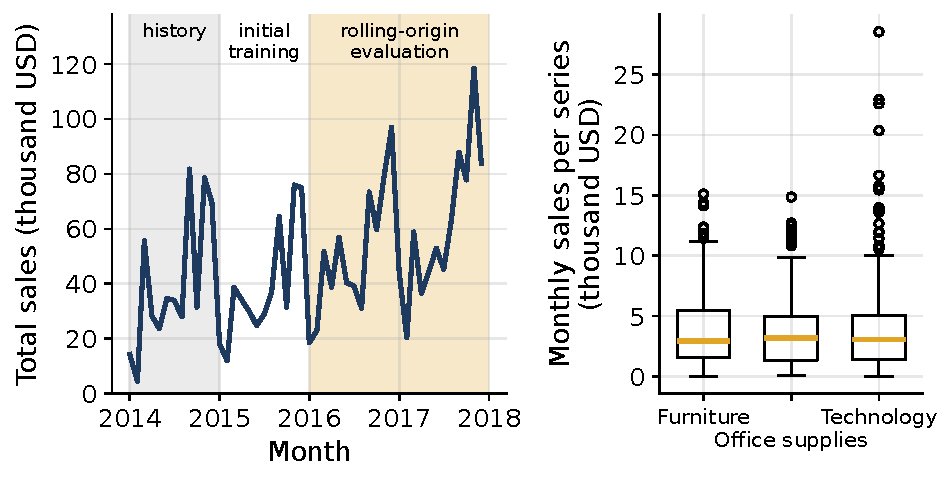
\includegraphics[width=\linewidth]{figures/eda_overview.pdf}
\caption{Izquierda: ventas mensuales totales de la empresa, con el año que solo aporta historia (2014), la ventana inicial de entrenamiento (2015) y el periodo de evaluación de origen móvil (2016--2017). Derecha: distribución de las ventas mensuales por serie en cada categoría; los puntos son valores atípicos.}
\label{fig:eda}
\end{figure}

\begin{figure}[!htb]
\centering
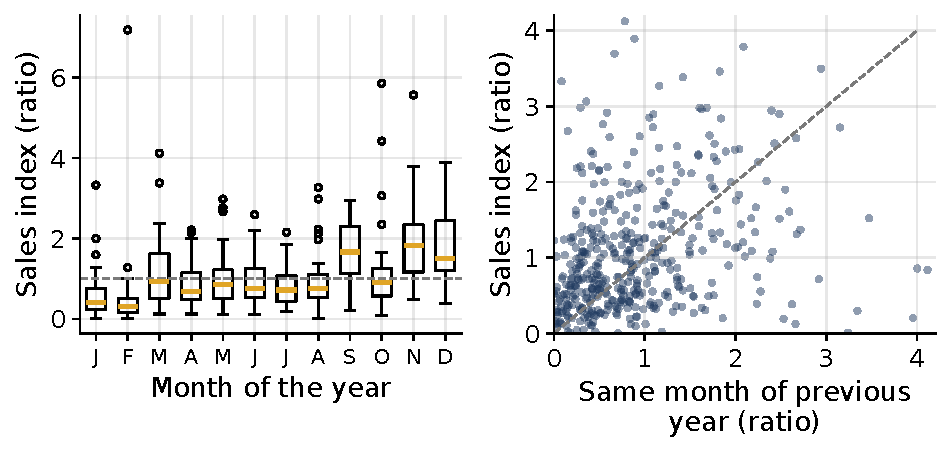
\includegraphics[width=\linewidth]{figures/eda_index.pdf}
\caption{Izquierda: distribución del índice de ventas por mes del año (2015--2017); la línea discontinua marca el nivel promedio de los doce meses previos. Derecha: índice de ventas frente a las ventas relativas del mismo mes del año anterior; la línea discontinua es la identidad.}
\label{fig:indice}
\end{figure}

\textbf{Decisiones derivadas del análisis exploratorio.} (i) El crecimiento de 2016--2017 y la diferencia de escala entre series motivan el índice de la Ecuación~\eqref{eq:indice}: dividir por el nivel reciente hace comparables las series y elimina la tendencia de la variable objetivo. (ii) Que el patrón estacional del índice sea común a las series motiva estimarlo con todas ellas agrupadas. (iii) Que el rezago anual de una serie sea un predictor ruidoso (un solo mes, con atípicos) motiva no usarlo tal cual, como hace el ingenuo estacional, sino contraerlo hacia el patrón común. (iv) Los atípicos son ventas reales y se conservan; por eso la métrica primaria es el MAE y no el error cuadrático. (v) Descuento, cantidad y utilidad no se conocen antes de que ocurra el mes y se excluyen para evitar fuga de información.

\subsection{Modelos de referencia (baselines)}\label{subsec:sota}

El modelo propuesto se compara con nueve referencias: el pronóstico ingenuo estacional y ocho regresores que cubren familias lineales, bayesianas, de vecinos, de árboles, de ensambles y de núcleo. Todos predicen el índice $z$ con las variables de la Ecuación~\eqref{eq:x}, el mismo preprocesamiento y las mismas particiones; sea $\mathcal{D}=\{(\mathbf{x}_i,z_i)\}_{i=1}^{n}$ la muestra de entrenamiento ya codificada.

El \textbf{ingenuo estacional} \cite{hyndman2021} no estima parámetros y representa la práctica actual de planificación:
\begin{equation}
\hat{y}_{s,t}=y_{s,t-12}.
\label{eq:naive}
\end{equation}
\textbf{Ridge} y \textbf{Lasso} ajustan un modelo lineal por mínimos cuadrados penalizados, con penalización $\ell_2$ y $\ell_1$ respectivamente \cite{hoerl1970,tibshirani1996}:
\begin{equation}
\hat{\boldsymbol{\beta}}=\arg\min_{\beta_0,\boldsymbol{\beta}}\sum_{i=1}^{n}\bigl(z_i-\beta_0-\mathbf{x}_i^{\top}\boldsymbol{\beta}\bigr)^2+\lambda R(\boldsymbol{\beta}),\qquad R(\boldsymbol{\beta})=\lVert\boldsymbol{\beta}\rVert_2^2\ \text{o}\ \lVert\boldsymbol{\beta}\rVert_1.
\label{eq:ridge}
\end{equation}
La \textbf{regresión bayesiana} (\texttt{BayesianRidge}) coloca una distribución a priori gaussiana sobre los coeficientes y estima las precisiones del ruido y de los pesos maximizando la verosimilitud marginal \cite{mackay1992}:
\begin{equation}
z_i\mid\mathbf{x}_i,\boldsymbol{\beta},\alpha\sim\mathcal{N}\bigl(\mathbf{x}_i^{\top}\boldsymbol{\beta},\alpha^{-1}\bigr),\qquad \boldsymbol{\beta}\mid\lambda\sim\mathcal{N}\bigl(\mathbf{0},\lambda^{-1}\mathbf{I}\bigr),
\label{eq:bayes}
\end{equation}
con distribuciones a priori Gamma sobre $\alpha$ y $\lambda$; el pronóstico es la media de la distribución predictiva. \textbf{KNN} promedia el índice de los $k$ vecinos más cercanos en distancia euclidiana \cite{cover1967}:
\begin{equation}
\hat{f}(\mathbf{x})=\frac{1}{k}\sum_{i\in\mathcal{N}_k(\mathbf{x})}z_i.
\label{eq:knn}
\end{equation}
El \textbf{árbol de decisión} particiona el espacio de variables de forma recursiva, eligiendo en cada nodo la variable $j$ y el umbral $u$ que minimizan la suma de cuadrados dentro de las dos regiones resultantes \cite{breiman1984}:
\begin{equation}
\min_{j,u}\Bigl[\sum_{i:\,x_{ij}\le u}\bigl(z_i-\bar{z}_{R_1}\bigr)^2+\sum_{i:\,x_{ij}>u}\bigl(z_i-\bar{z}_{R_2}\bigr)^2\Bigr].
\label{eq:arbol}
\end{equation}
\textbf{Random Forest} promedia $B$ árboles de regresión, cada uno crecido con el criterio de la Ecuación~\eqref{eq:arbol} sobre una muestra \emph{bootstrap} y considerando en cada nodo un subconjunto aleatorio de variables \cite{breiman2001}:
\begin{equation}
\hat{f}(\mathbf{x})=\frac{1}{B}\sum_{b=1}^{B}T_b(\mathbf{x};\Theta_b),
\label{eq:rf}
\end{equation}
donde $\Theta_b$ reúne la muestra y las variables sorteadas para el árbol $b$. \textbf{XGBoost} construye un ensamble aditivo de $M$ árboles, $\hat{z}_i=\sum_{m=1}^{M}f_m(\mathbf{x}_i)$, minimizando un objetivo regularizado \cite{chen2016}:
\begin{equation}
\mathcal{L}=\sum_{i=1}^{n}\bigl(z_i-\hat{z}_i\bigr)^2+\sum_{m=1}^{M}\Bigl(\gamma\,T_m+\tfrac{1}{2}\lambda\lVert\mathbf{w}_m\rVert_2^2\Bigr),
\label{eq:xgb}
\end{equation}
donde $T_m$ es el número de hojas del árbol $m$ y $\mathbf{w}_m$ sus pesos. La \textbf{regresión de vectores de soporte} (SVR) ajusta $f(\mathbf{x})=\mathbf{w}^{\top}\phi(\mathbf{x})+b$ bajo la pérdida insensible a $\varepsilon$ \cite{drucker1997}:
\begin{equation}
\min_{\mathbf{w},b}\ \tfrac{1}{2}\lVert\mathbf{w}\rVert_2^2+C\sum_{i=1}^{n}\max\bigl(0,\lvert z_i-f(\mathbf{x}_i)\rvert-\varepsilon\bigr),
\label{eq:svr}
\end{equation}
con núcleo gaussiano $K(\mathbf{x},\mathbf{x}')=\exp(-\gamma\lVert\mathbf{x}-\mathbf{x}'\rVert_2^2)$. Se usaron las implementaciones de scikit-learn 1.7.2 \cite{pedregosa2011} y XGBoost 3.2.0 \cite{chen2016}. La Tabla~\ref{tab:rejillas} lista las rejillas exploradas.

\begin{table}[!htb]
\caption{Rejillas de hiperparámetros exploradas con búsqueda exhaustiva y validación cruzada temporal. Los demás hiperparámetros conservan los valores por defecto de la librería.}\label{tab:rejillas}
\footnotesize
\begin{tabular*}{\textwidth}{@{\extracolsep\fill}p{0.24\textwidth}p{0.60\textwidth}c}
\toprule
Modelo & Rejilla & Config. \\
\midrule
Ridge & $\alpha\in\{0.01, 0.1, 1, 10, 100\}$ & 5 \\
Lasso & $\alpha\in\{10^{-4}, 10^{-3}, 10^{-2}, 10^{-1}\}$ & 4 \\
Regresión bayesiana & $\alpha_1,\lambda_1\in\{10^{-6}, 10^{-3}, 1\}$ & 9 \\
KNN & $k\in\{3, 5, 10, 15, 20, 30\}$; pesos uniformes o por distancia & 12 \\
Árbol de decisión & profundidad $\in\{2, 3, 4, 6\}$; mínimo por hoja $\in\{1, 5, 10, 20\}$ & 16 \\
Random Forest (300 árboles) & profundidad $\in\{3, 5, \text{sin límite}\}$; mínimo por hoja $\in\{1, 3, 5, 10\}$; fracción de variables $\in\{1, 0.5\}$ & 24 \\
XGBoost (300 árboles) & profundidad $\in\{2, 3, 4\}$; tasa $\in\{0.03, 0.1\}$; submuestra $\in\{0.8, 1\}$; peso mínimo de hijo $\in\{1, 5\}$ & 24 \\
SVR (núcleo RBF) & $C\in\{0.1, 1, 10\}$; $\varepsilon\in\{0.05, 0.1, 0.2\}$; $\gamma\in\{\text{scale}, 0.05\}$ & 18 \\
Modelo propuesto & $w\in\{0, 0.1, 0.2, 0.3, 0.4, 0.5\}$; perfil con media o mediana & 12 \\
\botrule
\end{tabular*}
\end{table}

\subsection{Modelo propuesto}\label{subsec:propuesto}

\textbf{Idea central.} El \emph{perfil estacional global contraído} predice el índice de ventas como una combinación de dos fuentes: el patrón estacional común, estimado con todas las series agrupadas, y lo que la propia serie vendió el mismo mes del año anterior. El resultado se devuelve a dólares con el nivel reciente de cada serie. La Figura~\ref{fig:metodo} muestra el flujo y el Algoritmo~\ref{alg:propuesto} el procedimiento.

\begin{figure}[!htb]
\centering
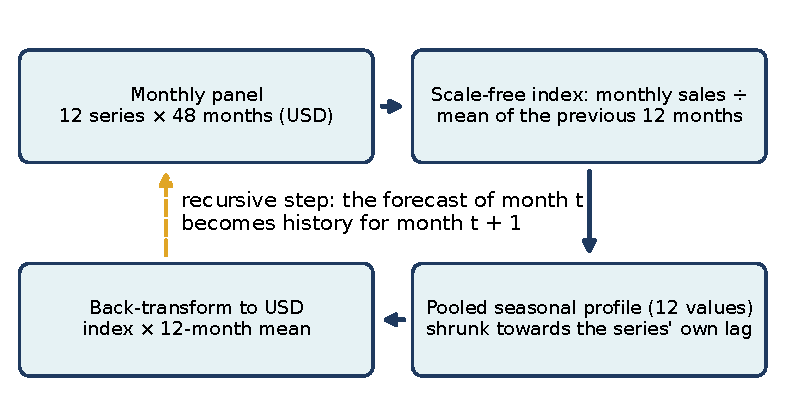
\includegraphics[width=\linewidth]{figures/method_diagram.pdf}
\caption{Flujo del modelo propuesto. El panel mensual en dólares se transforma en un índice libre de escala, el perfil estacional común se estima con las series agrupadas y se contrae hacia el rezago anual de cada serie, y el resultado se devuelve a dólares; en la proyección a varios meses, cada pronóstico se incorpora a la historia del mes siguiente.}
\label{fig:metodo}
\end{figure}

El perfil estacional es el valor típico del índice en cada mes del año, calculado sobre todas las series y todos los años de entrenamiento:
\begin{equation}
P_m=g\bigl(\{z_{s,t}: m_t=m,\ (s,t)\in\text{entrenamiento}\}\bigr),\qquad m=1,\dots,12,
\label{eq:perfil}
\end{equation}
donde $g$ es la media o la mediana. El pronóstico del índice es
\begin{equation}
\hat{z}_{s,t}=(1-w)\,P_{m_t}+w\,r^{(12)}_{s,t},\qquad w\in[0,1],
\label{eq:peg}
\end{equation}
y el pronóstico en dólares se obtiene con la Ecuación~\eqref{eq:retorno}. Con $w=1$ resulta $\hat{y}_{s,t}=y_{s,t-12}$, el ingenuo estacional de la Ecuación~\eqref{eq:naive}; con $w=0$, el nivel de la serie multiplicado por el perfil común. Para un horizonte $h>1$, las ventas aún no observadas se sustituyen por sus pronósticos al calcular el nivel y el rezago \cite{taieb2012}:
\begin{equation}
\hat{y}_{s,t+h}=\max\bigl(0,\;\hat{z}_{s,t+h}\,\tilde{\ell}_{s,t+h}\bigr),\qquad \tilde{y}_{s,u}=\begin{cases}y_{s,u}, & u\le t,\\ \hat{y}_{s,u}, & u>t,\end{cases}
\label{eq:recursivo}
\end{equation}
con $\tilde{\ell}$ y $r^{(12)}$ calculados sobre $\tilde{y}$.

\begin{algorithm}
\caption{Perfil estacional global contraído y proyección recursiva}\label{alg:propuesto}
\begin{algorithmic}[1]
\Require Panel $\{y_{s,t}\}$ hasta el mes $t_0$, rejilla $\mathcal{G}$ de pares $(w,g)$, horizonte $H$
\Ensure Pronósticos $\hat{y}_{s,t_0+h}$ para $h=1,\dots,H$ y toda serie $s$
\State Calcular $\ell_{s,t}$, $z_{s,t}$ y $r^{(12)}_{s,t}$ con la Ecuación~\eqref{eq:indice} para todo $t\le t_0$ con doce meses de historia
\For{cada configuración $(w,g)\in\mathcal{G}$}
    \State Estimar el MAE del índice con validación cruzada temporal
\EndFor
\State Con la configuración de menor MAE, calcular $P_1,\dots,P_{12}$ con la Ecuación~\eqref{eq:perfil} sobre las series agrupadas
\For{$h=1,\dots,H$}
    \State Calcular $\tilde{\ell}_{s,t_0+h}$ y $r^{(12)}_{s,t_0+h}$ con la historia observada y los pronósticos previos
    \State $\hat{y}_{s,t_0+h}\gets\max\bigl(0,\,[(1-w)P_{m}+w\,r^{(12)}_{s,t_0+h}]\,\tilde{\ell}_{s,t_0+h}\bigr)$, con $m$ el mes de $t_0+h$
    \State Añadir $\hat{y}_{s,t_0+h}$ a la historia de la serie $s$
\EndFor
\State \Return $\{\hat{y}_{s,t_0+h}\}$
\end{algorithmic}
\end{algorithm}

\textbf{Justificación de cada componente.} (a) \emph{Índice con nivel móvil:} traslada la tendencia al nivel $\ell_{s,t}$, que se actualiza cada mes, y deja al modelo la parte estacionaria; es la misma idea de los métodos globales que normalizan por la escala de la serie \cite{salinas2020,smyl2020}. (b) \emph{Perfil común (agrupación):} cada serie aporta uno o dos datos por mes del año, insuficientes para estimar su propia estacionalidad; con doce series el perfil se apoya en doce veces más observaciones, lo que es razonable cuando las series comparten calendario \cite{monteromanso2021}. (c) \emph{Contracción hacia la serie:} el peso $w$ permite que cada serie se aparte del patrón común según lo que ella misma hizo un año antes, y hace del ingenuo estacional un caso límite del modelo. (d) \emph{Media o mediana:} la mediana minimiza el error absoluto, pero la media reproduce el total; se deja que la validación cruzada elija y el efecto se examina en la ablación. Frente a los regresores generales, la apuesta es de sesgo y varianza: con pocas observaciones ruidosas, un modelo de doce parámetros tiene mucha menos varianza que un ensamble, y si la estructura que impone es la correcta su sesgo es pequeño.

\textbf{Complejidad.} El ajuste recorre los datos una vez para agruparlos por mes: $\mathcal{O}(n)$ en tiempo con la media ($\mathcal{O}(n\log n)$ con la mediana) y $\mathcal{O}(1)$ en memoria, pues el modelo son 12 números. La predicción es una consulta y una combinación lineal, $\mathcal{O}(1)$ por observación. Como comparación, el Random Forest ajustado en este estudio ocupa, serializado, unas 2{,}500 veces más.

\textbf{Qué es nuevo y qué se reutiliza.} Los ingredientes son conocidos: los índices estacionales y el ingenuo estacional son clásicos \cite{hyndman2021}, la normalización por nivel y el entrenamiento global provienen de la literatura reciente \cite{salinas2020,monteromanso2021} y la estrategia recursiva de \cite{taieb2012}. El aporte es su combinación en un estimador mínimo que contiene al ingenuo estacional como caso particular, y la evidencia de que, en un panel pequeño, compite con ensambles cientos de veces más costosos.

\textbf{Origen del diseño.} El modelo se concibió después de analizar una primera versión del estudio, en la que la importancia de variables de un Random Forest evaluado sobre 2017 mostró que la señal estaba en el mes del año y en el rezago anual. El diseño, la rejilla y el protocolo de evaluación se fijaron antes de calcular el desempeño del modelo, que se evaluó una sola vez; pero la idea se benefició de datos que forman parte de la evaluación, lo que se declara como limitación.

\subsection{Entrenamiento y optimización}\label{subsec:entrenamiento}

Los hiperparámetros de todos los modelos se ajustan con búsqueda exhaustiva en rejilla (\texttt{GridSearchCV}) y validación cruzada temporal (\texttt{TimeSeriesSplit}) con pliegues de validación de tres meses (36 filas) posteriores a su ventana de entrenamiento. El criterio es el MAE del índice, Ecuación~\eqref{eq:perdida}. El codificador y el escalador de los modelos de referencia se reajustan dentro de cada pliegue. Las rejillas tienen entre 4 y 24 configuraciones (Tabla~\ref{tab:rejillas}); el modelo propuesto explora 12, menos que el árbol de decisión, Random Forest, XGBoost y SVR, y ningún modelo usa valores por defecto sin búsqueda. El modelo propuesto no tiene épocas, tasa de aprendizaje, parada temprana ni componente aleatorio. Random Forest y XGBoost usan 300 árboles y semilla 42. El conjunto evaluado nunca interviene en la selección: en cada origen, la búsqueda usa solo meses anteriores.

\subsection{Protocolo de evaluación}\label{subsec:evaluacion}

\textbf{Protocolo primario: origen móvil.} Se usan 24 orígenes mensuales, de enero de 2016 a diciembre de 2017 \cite{cerqueira2020}. En cada origen $t$, todos los modelos se reentrenan con los meses anteriores (ventana creciente desde enero de 2015, de 12 a 35 meses), reajustan sus hiperparámetros con validación cruzada anidada dentro de esa ventana y pronostican el mes $t$ de las 12 series, lo que da 288 pronósticos a un paso en 24 bloques mensuales. La validación interna usa hasta 4 pliegues de tres meses, dejando al menos seis meses de entrenamiento en el primero (2 pliegues con 12 a 14 meses, 3 con 15 a 17 y 4 en adelante).

\textbf{Protocolo secundario: partición fija.} Para mantener la comparación con la partición original del proyecto, los modelos se ajustan con 2015--2016 (4 pliegues trimestrales sobre 2016) y se evalúan en 2017 sin reentrenar, a un paso y con una \emph{proyección recursiva a doce meses} que, con el Algoritmo~\ref{alg:propuesto} y datos hasta 2016, proyecta todo 2017 como se haría con el año siguiente.

\textbf{Métricas.} La métrica primaria es el MAE en dólares por serie y mes. Las secundarias son la raíz del error cuadrático medio (RMSE), el error porcentual absoluto ponderado (WAPE), el error absoluto escalado (MASE) \cite{hyndman2006}, el coeficiente $R^2$ y el desvío del total:
\begin{gather}
\mathrm{WAPE}=\frac{\sum_{s,t}\lvert e_{s,t}\rvert}{\sum_{s,t}y_{s,t}},\qquad
\Delta_{\mathrm{total}}=\frac{\sum_{s,t}\hat{y}_{s,t}}{\sum_{s,t}y_{s,t}}-1,\notag\\
\mathrm{MASE}=\frac{\frac{1}{n_{\mathrm{ev}}}\sum_{(s,t)\in\mathrm{ev}}\lvert e_{s,t}\rvert}{\frac{1}{n_0}\sum_{(s,t)\in 2015}\lvert y_{s,t}-y_{s,t-12}\rvert}.
\label{eq:metricas}
\end{gather}
El MASE se escala con el error del ingenuo estacional en 2015, el periodo anterior al primer origen. Se usa WAPE en lugar de MAPE porque hay meses con ventas cercanas a cero que vuelven inestable el error porcentual individual.

\textbf{Incertidumbre.} La variabilidad se reporta como media $\pm$ desviación estándar del MAE sobre los 24 bloques mensuales y con intervalos de confianza del 95\% por \emph{bootstrap} de bloques móviles circulares \cite{kunsch1989} de tres meses y 10{,}000 remuestras.

\textbf{Pruebas de significancia.} Se sigue la combinación recomendada para pronóstico de series de tiempo; la prueba $t$ con varianza corregida \cite{nadeau2003} no se usa porque supone particiones intercambiables. Para cada referencia $b$ se define el diferencial de pérdida absoluta promediado sobre las series, lo que absorbe la dependencia entre series de un mismo mes:
\begin{equation}
d_t=\frac{1}{S}\sum_{s=1}^{S}\bigl(\lvert e^{\mathrm{prop}}_{s,t}\rvert-\lvert e^{b}_{s,t}\rvert\bigr),\qquad t=1,\dots,24,
\label{eq:dt}
\end{equation}
con valores negativos a favor del modelo propuesto. (1) La prueba de \emph{Diebold--Mariano} \cite{diebold1995} con la corrección de Harvey--Leybourne--Newbold \cite{harvey1997} contrasta $\mathbb{E}[d_t]=0$ con el estadístico $\sqrt{(T-1)/T}\;\bar{d}/\sqrt{\hat{\gamma}_0/T}$ para horizonte 1, comparado con una $t_{T-1}$; se repite con pérdida cuadrática como comprobación. (2) La prueba de \emph{Giacomini--White} \cite{giacomini2006} de capacidad predictiva condicional, apropiada para modelos reestimados en ventanas finitas, usa los instrumentos $\mathbf{h}_t=(1,d_t)^{\top}$ y el estadístico $n\,\bar{\mathbf{Z}}^{\top}\hat{\boldsymbol{\Omega}}^{-1}\bar{\mathbf{Z}}\sim\chi^2_2$, con $\mathbf{Z}_{t+1}=\mathbf{h}_t d_{t+1}$ y $n=23$. (3) La prueba $t$ \emph{correlacionada bayesiana} \cite{corani2015,benavoli2017} sobre el MAE mensual estima la probabilidad posterior de que el modelo propuesto sea mejor, equivalente o peor respecto de una región de equivalencia práctica (ROPE) de $\pm1$\% de la venta media anterior al primer origen ($\pm32.68$ USD), con correlación $\rho=1/24$; por la dependencia temporal se interpreta con cautela. Como comprobación no paramétrica se añade la prueba de rangos con signo de Wilcoxon. Los valores $p$ de los $m=9$ contrastes se ajustan con el método de Holm \cite{holm1979} por separado para cada prueba, con $\alpha=0.05$. Cada contraste se acompaña de la diferencia media de MAE con su intervalo de confianza y de la $d$ de Cohen de las diferencias pareadas. La prueba de Friedman no se aplica porque hay un solo conjunto de datos.

\subsection{Diseño del estudio de ablación}\label{subsec:ablacion}

Cada variante elimina o reemplaza un componente del modelo completo y mantiene lo demás: mismo protocolo de origen móvil, misma validación anidada, mismas métricas y mismas pruebas. Las hipótesis son: (H1) \emph{sin perfil estacional}, con $P_m$ constante: el error aumenta porque se pierde el patrón de calendario; (H2) \emph{sin rezago de la serie}, con $w=0$: el error aumenta porque se pierde la información propia de cada serie; (H3) \emph{sin agrupar}, con un perfil por serie: el error aumenta porque cada perfil se estima con uno a tres datos por mes; (H4) \emph{sin nivel móvil}, con el nivel fijo en la media de toda la historia previa de la serie: el error aumenta y el total se subestima, porque el nivel deja de seguir el crecimiento; (H5) \emph{mediana en lugar de media}: el error absoluto baja y el total se subestima, por la asimetría del índice.

\subsection{Configuración experimental y disponibilidad}\label{subsec:config}

Los experimentos se ejecutaron en un computador portátil con procesador AMD Ryzen 5 7520U (4 núcleos, 8 hilos), 8 GB de memoria RAM y Windows 11, sin GPU, con Python 3.10.11, scikit-learn 1.7.2, XGBoost 3.2.0, pandas 2.3.3, NumPy 2.2.6, SciPy 1.15.3 y statsmodels 0.15.0. En cada origen se midieron tres tiempos: la búsqueda completa en rejilla (en paralelo para las referencias, secuencial para el modelo propuesto), el reajuste de la configuración seleccionada (mediana de 3 repeticiones, un hilo) y la predicción de las 12 filas del mes (mediana de 10 repeticiones); se reporta la mediana sobre los 24 orígenes y, como indicador de memoria, el tamaño del modelo serializado. El código, los datos y las versiones exactas de las librerías están en el repositorio indicado en las Declaraciones; el script \texttt{paper/experimentos.py} reproduce todas las tablas, pruebas y figuras de este artículo.

\section{Resultados}\label{sec:resultados}

\subsection{Resumen del montaje experimental}\label{subsec:montaje}

Se evalúan diez métodos sobre 288 pronósticos a un paso (12 series, 24 orígenes mensuales de 2016 y 2017), con reentrenamiento y reajuste de hiperparámetros en cada origen. La métrica primaria es el MAE en dólares; las secundarias son RMSE, WAPE, MASE, $R^2$ y el desvío del total. La incertidumbre se mide sobre los 24 bloques mensuales. La partición fija de 2017 se reporta como protocolo secundario.

\subsection{Desempeño predictivo global}\label{subsec:global}

La Tabla~\ref{tab:resultados} resume el desempeño. El modelo propuesto obtiene el mejor valor en seis de las ocho columnas: MAE (y sus reescalados WAPE y MASE), RMSE, $R^2$ y el MAE de 2016. Su MAE es 421 USD menor que el del ingenuo estacional (15.4\%), 116 USD menor que el de Random Forest (4.8\%) y 59 USD menor que el de SVR (2.5\%), el segundo mejor; es además el único método con MASE inferior a 1. En las otras dos columnas no gana: en 2017 queda segundo detrás de SVR y en el desvío del total queda cuarto ($-5.8$\%, frente a $-3.2$\% de XGBoost). Su variabilidad entre meses es intermedia (Figura~\ref{fig:box}).

\begin{table}[!htb]
\caption{Desempeño en la evaluación de origen móvil (24 orígenes, 288 pronósticos a un paso). MAE: media $\pm$ desviación estándar sobre los 24 bloques mensuales. $\Delta_{\mathrm{total}}$: desvío del total de ventas del periodo. MAE$_{2016}$ y MAE$_{2017}$: MAE de los orígenes de cada año. En negrita el mejor valor de cada columna y subrayado el segundo.}\label{tab:resultados}
\footnotesize
\begin{tabular*}{\textwidth}{@{\extracolsep\fill}lrrrrrrrr}
\toprule
Modelo & MAE (USD) & RMSE & WAPE (\%) & MASE & $R^2$ & $\Delta_{\mathrm{total}}$ (\%) & MAE$_{2016}$ & MAE$_{2017}$ \\
\midrule
Ingenuo estacional & 2{,}728 $\pm$ 928 & 4{,}050 & 58.5 & 1.176 & $-0.098$ & $-19.6$ & 2{,}543 & 2{,}912 \\
Ridge & 2{,}517 $\pm$ 878 & 3{,}508 & 54.0 & 1.085 & 0.176 & $-6.0$ & 2{,}323 & 2{,}710 \\
Lasso & 2{,}528 $\pm$ 867 & 3{,}507 & 54.2 & 1.090 & 0.177 & $-6.7$ & 2{,}330 & 2{,}726 \\
Regresión bayesiana & 2{,}523 $\pm$ 866 & 3{,}513 & 54.1 & 1.088 & 0.174 & $-7.4$ & 2{,}356 & 2{,}690 \\
KNN & 2{,}453 $\pm$ 936 & 3{,}495 & 52.6 & 1.057 & 0.182 & \underline{$-5.3$} & 2{,}236 & 2{,}670 \\
Árbol de decisión & 2{,}529 $\pm$ 841 & 3{,}647 & 54.3 & 1.090 & 0.110 & $-7.8$ & 2{,}327 & 2{,}732 \\
Random Forest & 2{,}423 $\pm$ 785 & \underline{3{,}489} & 52.0 & 1.044 & \underline{0.185} & $-5.4$ & \underline{2{,}181} & 2{,}665 \\
XGBoost & 2{,}523 $\pm$ 849 & 3{,}654 & 54.1 & 1.088 & 0.106 & $\mathbf{-3.2}$ & 2{,}291 & 2{,}755 \\
SVR & \underline{2{,}366} $\pm$ 913 & 3{,}531 & \underline{50.8} & \underline{1.020} & 0.166 & $-18.2$ & 2{,}288 & \textbf{2{,}444} \\
Modelo propuesto & \textbf{2{,}307} $\pm$ 846 & \textbf{3{,}436} & \textbf{49.5} & \textbf{0.994} & \textbf{0.210} & $-5.8$ & \textbf{2{,}054} & \underline{2{,}559} \\
\botrule
\end{tabular*}
\footnotetext{La significancia de las diferencias frente al modelo propuesto se reporta en la Tabla~\ref{tab:pruebas}: tras la corrección de Holm, la prueba de Diebold--Mariano respalda la diferencia frente al ingenuo estacional y XGBoost.}
\end{table}

\begin{figure}[!htb]
\centering
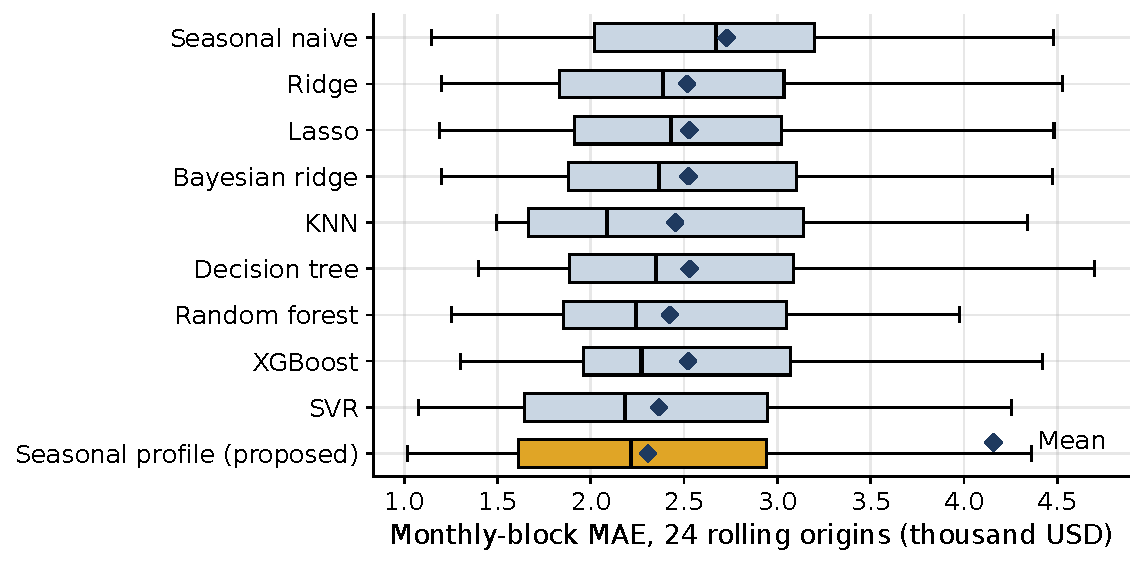
\includegraphics[width=\linewidth]{figures/mae_boxplot.pdf}
\caption{Distribución del MAE de los 24 bloques mensuales de la evaluación de origen móvil para cada modelo. El rombo indica la media, que coincide con el MAE global de la Tabla~\ref{tab:resultados}.}
\label{fig:box}
\end{figure}

Todos los modelos subestiman el total del periodo, porque el nivel de doce meses va por detrás de una serie que crece; los modelos sobre el índice lo hacen entre 3\% y 8\%, mientras que el ingenuo estacional y SVR lo subestiman en casi una quinta parte. El $R^2$ de 0.21 indica que, a nivel de serie y mes, incluso el mejor modelo explica una fracción pequeña de la variabilidad: la Figura~\ref{fig:pred} muestra pronósticos concentrados por debajo de 15{,}000 USD frente a observaciones que superan los 20{,}000 USD. El desempeño mejora al agregar: sobre el total mensual de la empresa el WAPE del modelo propuesto es 21.2\%, frente a 25.0\% del ingenuo estacional (Figura~\ref{fig:serie}).

\begin{figure}[!htb]
\centering
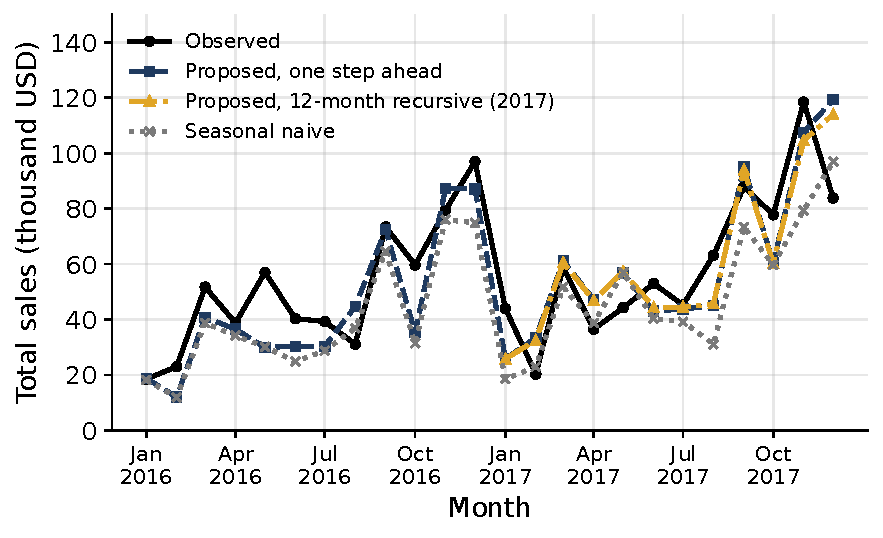
\includegraphics[width=\linewidth]{figures/forecast_total.pdf}
\caption{Ventas totales mensuales de 2016 y 2017: observadas, pronosticadas por el modelo propuesto a un paso en la evaluación de origen móvil, proyectadas de forma recursiva a doce meses para 2017 con datos hasta 2016, y pronóstico ingenuo estacional.}
\label{fig:serie}
\end{figure}

\begin{figure}[!htb]
\centering
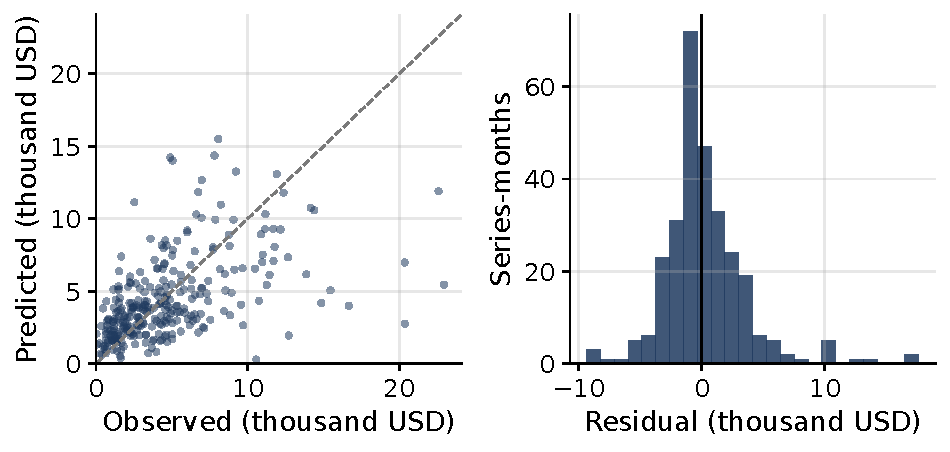
\includegraphics[width=\linewidth]{figures/pred_vs_obs.pdf}
\caption{Modelo propuesto en la evaluación de origen móvil. Izquierda: ventas pronosticadas frente a observadas por serie y mes; la línea discontinua es la identidad. Derecha: distribución de los residuos (observado menos pronosticado).}
\label{fig:pred}
\end{figure}

\textbf{Partición fija de 2017.} La Tabla~\ref{tab:fija} muestra el protocolo secundario. Sin reentrenamiento y con solo doce bloques, el modelo propuesto es segundo en MAE a un paso y en la proyección recursiva, en ambos casos detrás de SVR, y es el que menos desvía el total anual proyectado a doce meses ($-0.4$\%); SVR lo subestima en 13.8\%. Ninguna diferencia frente al modelo propuesto es significativa en esta partición ($p_{\mathrm{Holm}}=1.000$ en todos los contrastes): frente a SVR la diferencia de MAE es de $+48$ USD, con intervalo [$-270$, 378].

\begin{table}[!htb]
\caption{Protocolo secundario: modelos ajustados con 2015--2016 y evaluados en 2017 sin reentrenar (144 observaciones). MAE: media $\pm$ desviación estándar sobre doce bloques mensuales. $\Delta_1$ y $\Delta_{12}$: desvío del total anual a un paso y con proyección recursiva a doce meses; MAE$_{12}$: MAE de la proyección recursiva. En negrita el mejor valor de cada columna y subrayado el segundo.}\label{tab:fija}
\footnotesize
\begin{tabular*}{\textwidth}{@{\extracolsep\fill}lrrrr}
\toprule
Modelo & MAE (USD) & $\Delta_1$ (\%) & MAE$_{12}$ (USD) & $\Delta_{12}$ (\%) \\
\midrule
Ingenuo estacional & 2{,}912 $\pm$ 911 & $-16.9$ & 2{,}912 & $-16.9$ \\
Ridge & 2{,}708 $\pm$ 962 & $-1.6$ & 2{,}671 & $+4.1$ \\
Lasso & 2{,}698 $\pm$ 983 & $-1.6$ & 2{,}633 & \underline{$+2.9$} \\
Regresión bayesiana & 2{,}709 $\pm$ 959 & $-1.6$ & 2{,}674 & $+4.4$ \\
KNN & 2{,}757 $\pm$ 1{,}128 & $+2.2$ & 2{,}933 & $+11.1$ \\
Árbol de decisión & 2{,}635 $\pm$ 973 & $\mathbf{+0.6}$ & 2{,}537 & $+3.5$ \\
Random Forest & 2{,}634 $\pm$ 834 & \underline{$+0.7$} & 2{,}609 & $+3.4$ \\
XGBoost & 2{,}672 $\pm$ 906 & $+1.7$ & 2{,}908 & $+10.4$ \\
SVR & \textbf{2{,}511} $\pm$ 1{,}017 & $-13.8$ & \textbf{2{,}370} & $-13.8$ \\
Modelo propuesto & \underline{2{,}559} $\pm$ 927 & $+0.7$ & \underline{2{,}490} & $\mathbf{-0.4}$ \\
\botrule
\end{tabular*}
\end{table}

\subsection{Resultados de las pruebas de significancia}\label{subsec:pruebas}

La Tabla~\ref{tab:pruebas} y la Figura~\ref{fig:dif} presentan los contrastes del protocolo primario. Con la prueba de Diebold--Mariano, el modelo propuesto supera significativamente a 2 de las 9 referencias tras la corrección de Holm, el ingenuo estacional ($p_{\mathrm{Holm}}=0.025$) y XGBoost ($p_{\mathrm{Holm}}=0.034$), y no se distingue estadísticamente de las otras 7. La diferencia media favorece al modelo propuesto en los nueve contrastes, y en siete de ellos el intervalo de confianza del 95\% excluye el cero; las excepciones son KNN y SVR.

\begin{table}[!htb]
\caption{Contrastes del modelo propuesto frente a cada referencia en la evaluación de origen móvil ($T=24$ bloques mensuales). $\Delta$MAE: diferencia media propuesto menos referencia, en USD, con intervalo de confianza del 95\% por \emph{bootstrap} de bloques (valores negativos favorecen al propuesto). $d$: $d$ de Cohen de las diferencias pareadas. DM: Diebold--Mariano con corrección HLN y pérdida absoluta; GW: Giacomini--White; entre paréntesis, valor $p$ sin ajustar y ajustado por Holm ($m=9$). Bayes: probabilidad posterior de que el propuesto sea mejor / equivalente dentro de la ROPE / peor. Meses: bloques, de 24, en que el propuesto tiene menor MAE.}\label{tab:pruebas}
\scriptsize
\begin{tabular*}{\textwidth}{@{\extracolsep\fill}lrrrrrr}
\toprule
Referencia & $\Delta$MAE [IC 95\%] & $d$ & DM ($p$; $p_{\mathrm{Holm}}$) & GW ($p$; $p_{\mathrm{Holm}}$) & Bayes & Meses \\
\midrule
Ingenuo estacional & $-421$ [$-626$, $-181$] & $-0.69$ & $-3.36$ (0.003; 0.025) & 7.51 (0.023; 0.210) & 0.98 / 0.01 / 0.01 & 18 \\
Ridge & $-210$ [$-408$, $-14$] & $-0.35$ & $-1.72$ (0.098; 0.433) & 2.20 (0.334; 1.000) & 0.84 / 0.07 / 0.09 & 16 \\
Lasso & $-222$ [$-442$, $-9$] & $-0.35$ & $-1.73$ (0.097; 0.433) & 2.24 (0.326; 1.000) & 0.84 / 0.07 / 0.09 & 18 \\
Regresión bayesiana & $-216$ [$-409$, $-14$] & $-0.37$ & $-1.79$ (0.086; 0.433) & 2.51 (0.284; 1.000) & 0.85 / 0.07 / 0.08 & 16 \\
KNN & $-146$ [$-352$, 36] & $-0.28$ & $-1.38$ (0.182; 0.433) & 2.30 (0.317; 1.000) & 0.77 / 0.11 / 0.12 & 15 \\
Árbol de decisión & $-223$ [$-364$, $-71$] & $-0.48$ & $-2.36$ (0.027; 0.192) & 5.12 (0.078; 0.542) & 0.91 / 0.05 / 0.04 & 17 \\
Random Forest & $-116$ [$-221$, $-17$] & $-0.44$ & $-2.16$ (0.041; 0.246) & 4.37 (0.113; 0.676) & 0.86 / 0.11 / 0.03 & 16 \\
XGBoost & $-216$ [$-364$, $-77$] & $-0.65$ & $-3.17$ (0.004; 0.034) & 6.84 (0.033; 0.261) & 0.96 / 0.03 / 0.01 & 20 \\
SVR & $-59$ [$-226$, 153] & $-0.11$ & $-0.53$ (0.599; 0.599) & 0.25 (0.882; 1.000) & 0.56 / 0.15 / 0.28 & 15 \\
\botrule
\end{tabular*}
\end{table}

\begin{figure}[!htb]
\centering
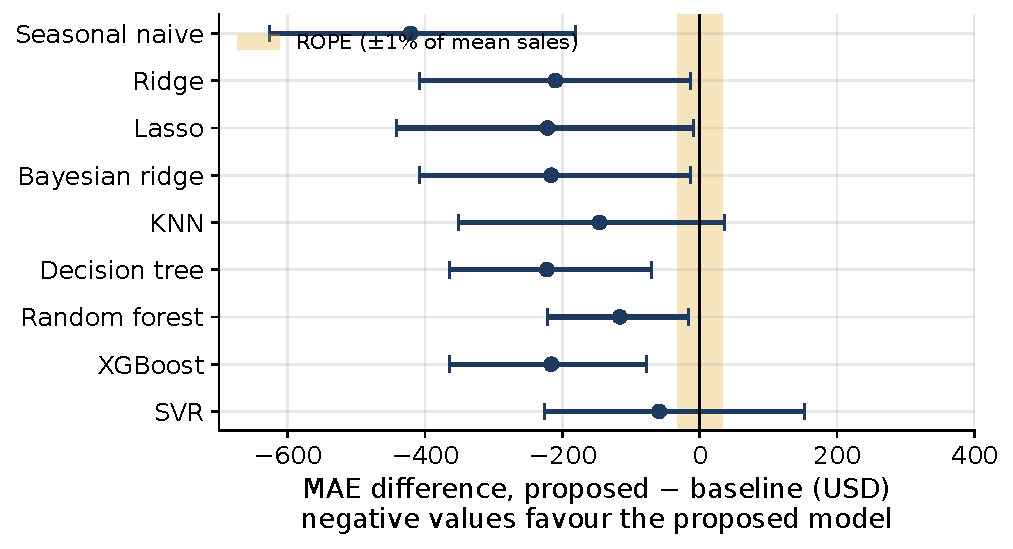
\includegraphics[width=\linewidth]{figures/mae_differences.pdf}
\caption{Diferencia media de MAE entre el modelo propuesto y cada referencia en la evaluación de origen móvil, con intervalo de confianza del 95\% por \emph{bootstrap} de bloques. La franja sombreada es la región de equivalencia práctica ($\pm1$\% de la venta media).}
\label{fig:dif}
\end{figure}

Los tamaños de efecto ordenan la evidencia. Frente al ingenuo estacional y XGBoost el efecto es mediano ($d=-0.69$ y $-0.65$) y la probabilidad posterior de que el modelo propuesto sea mejor es de 0.98 y 0.96. Frente al árbol de decisión y Random Forest el efecto es entre pequeño y mediano ($d=-0.48$ y $-0.44$), los valores $p$ sin ajustar son 0.027 y 0.041 y las probabilidades posteriores 0.91 y 0.86, pero la corrección por nueve comparaciones los deja en 0.192 y 0.246: hay indicios de mejora, no evidencia concluyente. Frente a los tres modelos lineales el efecto es pequeño ($d\approx-0.35$). Frente a KNN y SVR la ventaja es la menor (146 y 59 USD), con probabilidades de 0.77 y 0.56; con SVR el modelo propuesto es, a efectos estadísticos, equivalente en MAE.

Las pruebas no coinciden del todo y conviene decir por qué. Giacomini--White no rechaza en ningún contraste tras Holm (el menor $p_{\mathrm{Holm}}$ es 0.210), aunque sin ajustar señala a las mismas dos referencias que Diebold--Mariano (0.023 y 0.033): contrasta una hipótesis conjunta con dos grados de libertad y 23 observaciones, por lo que tiene menos potencia para una diferencia que es sobre todo de nivel medio. Con pérdida cuadrática, Diebold--Mariano solo conserva la diferencia frente al ingenuo estacional ($p_{\mathrm{Holm}}=0.029$), porque los errores grandes, que el modelo propuesto no evita, dominan esa pérdida. La prueba de Wilcoxon, añadida porque las diferencias mensuales no son normales frente a Ridge, Lasso, regresión bayesiana y SVR (Shapiro--Wilk, $p<0.01$), da $p<0.05$ sin ajustar frente a siete referencias y, tras Holm, frente a las mismas dos ($p_{\mathrm{Holm}}=0.028$). En cuanto a la relevancia práctica, las diferencias que favorecen al modelo van de 1.3\% a 9\% de la venta media por serie y mes (4{,}661 USD): pequeñas para un pronóstico individual, pero obtenidas con un modelo más simple y sin costo adicional.

\subsection{Resultados del estudio de ablación}\label{subsec:res_ablacion}

La Tabla~\ref{tab:ablacion} y la Figura~\ref{fig:abl} muestran las variantes.

\begin{table}[!htb]
\caption{Estudio de ablación en la evaluación de origen móvil. $\Delta$MAE: modelo completo menos variante, en USD, con intervalo de confianza del 95\% (valores negativos indican que quitar el componente empeora). $p_{\mathrm{Holm}}$: Diebold--Mariano con corrección HLN ($m=5$). Bayes: probabilidad posterior de que el modelo completo sea mejor / equivalente / peor. $\Delta_{\mathrm{total}}$: desvío del total.}\label{tab:ablacion}
\scriptsize
\begin{tabular*}{\textwidth}{@{\extracolsep\fill}lrrrrr}
\toprule
Variante & MAE (USD) & $\Delta$MAE [IC 95\%] & $p_{\mathrm{Holm}}$ & Bayes & $\Delta_{\mathrm{total}}$ (\%) \\
\midrule
Modelo completo & 2{,}307 $\pm$ 846 & -- & -- & -- & $-5.8$ \\
Sin perfil estacional, $P_m$ constante (H1) & 2{,}439 $\pm$ 879 & $-133$ [$-324$, 82] & 0.587 & 0.72 / 0.11 / 0.17 & $-14.0$ \\
Sin rezago de la serie, $w=0$ (H2) & 2{,}280 $\pm$ 860 & $+27$ [$-3$, 64] & 0.587 & 0.03 / 0.55 / 0.42 & $-4.6$ \\
Sin agrupar, perfil por serie (H3) & 2{,}801 $\pm$ 902 & $-494$ [$-715$, $-297$] & 0.002 & 0.99 / 0.00 / 0.00 & $-11.0$ \\
Sin nivel móvil, nivel estático (H4) & 2{,}185 $\pm$ 878 & $+122$ [$-19$, 291] & 0.585 & 0.10 / 0.13 / 0.78 & $-25.4$ \\
Mediana en lugar de media (H5) & 2{,}316 $\pm$ 854 & $-10$ [$-96$, 87] & 0.849 & 0.38 / 0.34 / 0.28 & $-17.3$ \\
\botrule
\end{tabular*}
\end{table}

\begin{figure}[!htb]
\centering
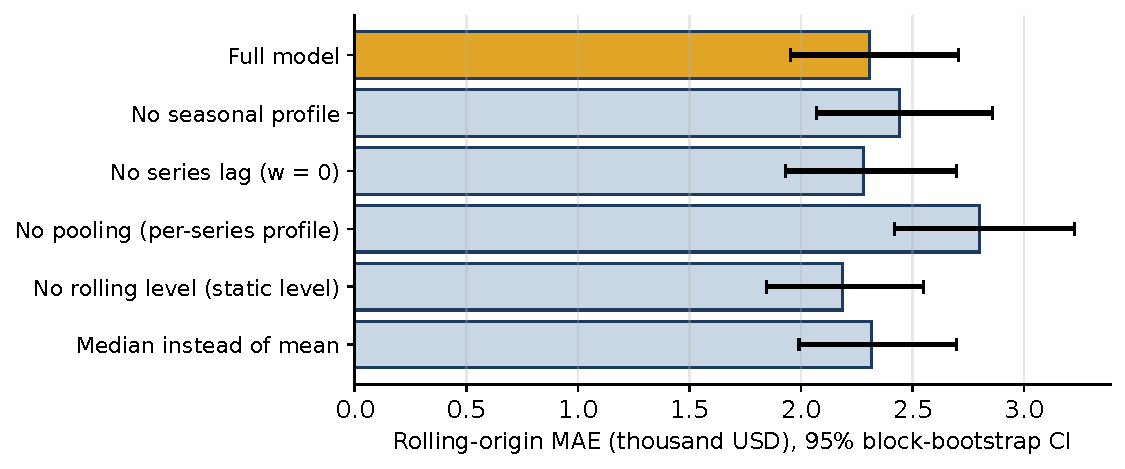
\includegraphics[width=\linewidth]{figures/ablation.pdf}
\caption{MAE del modelo completo y de cada variante de la ablación en la evaluación de origen móvil, con intervalos de confianza del 95\% por \emph{bootstrap} de bloques.}
\label{fig:abl}
\end{figure}

\emph{H3 (agrupación)} se confirma con claridad y es el único efecto significativo: estimar un perfil por serie eleva el MAE en 494 USD ($p_{\mathrm{Holm}}=0.002$ con Diebold--Mariano y 0.030 con Giacomini--White), hasta un error peor que el del ingenuo estacional. Agrupar las series es el componente del que depende el modelo. \emph{H1 (perfil estacional)} va en la dirección esperada sin alcanzar significancia: con un perfil constante el MAE sube 133 USD y el total se subestima en 14.0\%. \emph{H2 (rezago de la serie)} se refuta: con $w=0$ el error es 27 USD \emph{menor} y la mayor masa posterior cae en la ROPE (0.55); el componente es prescindible y el modelo más simple, nivel por perfil común, rinde igual.

\emph{H4 (nivel móvil)} se refuta en su primera parte y se confirma en la segunda: con nivel estático el MAE es 122 USD menor (intervalo [$-19$, 291]), pero el total se subestima en 25.4\%. \emph{H5 (mediana)} se confirma solo en el sesgo: el MAE no cambia (10 USD) y el total se subestima en 17.3\%. Los dos resultados describen el mismo intercambio: con ventas asimétricas a la derecha, un pronóstico que apunta por debajo acierta más meses corrientes y reduce el error absoluto, a costa de quedarse corto en el total. El nivel móvil y la media no mejoran el error por serie; lo que hacen es mantener el pronóstico cerca del nivel real de ventas. El mismo patrón explica el comportamiento de SVR en la Tabla~\ref{tab:resultados}.

\subsection{Sensibilidad y robustez}\label{subsec:sensibilidad}

\textbf{Semillas.} El modelo propuesto es determinista: no tiene componente aleatorio y su resultado no depende de ninguna semilla.

\textbf{Hiperparámetros.} La Figura~\ref{fig:sens} (izquierda) muestra el MAE de origen móvil con cada configuración fija. La curva es plana para $w\le0.2$ (entre 2{,}276 y 2{,}280 USD con la media) y crece hasta el error del ingenuo estacional en $w=1$; el desvío del total empeora de forma lineal con $w$, de $-4.6$\% a $-19.6$\%. Media y mediana dan prácticamente el mismo MAE para todo $w$, pero la mediana desvía el total entre $-17.6$\% y $-19.6$\%. La selección anidada (2{,}307 USD) queda 31 USD por encima de la mejor configuración fija, el costo de elegir sin ver el futuro. A lo largo de los orígenes, la validación eligió siempre la media, con $w=0.4$ cuando había 12 a 14 meses de entrenamiento, valores decrecientes después y $w=0$ desde los 23 meses: cuanta más historia hay para estimar el perfil, menos pesa el rezago individual.

\textbf{Tamaño de entrenamiento.} Al limitar la ventana a los últimos 12 o 18 meses, el MAE sube a 2{,}428 y 2{,}417 USD; con 24 meses es 2{,}284 USD, similar al de la ventana completa (Figura~\ref{fig:sens}, derecha). El modelo supera al ingenuo estacional con cualquier ventana, incluso con un solo año de datos.

\textbf{Robustez por periodo.} En 2016 el modelo propuesto es el mejor por 127 USD sobre Random Forest; en 2017 queda segundo, 115 USD por encima de SVR. La ventaja global no proviene de un solo año, pero su margen sí depende del periodo.

\begin{figure}[!htb]
\centering
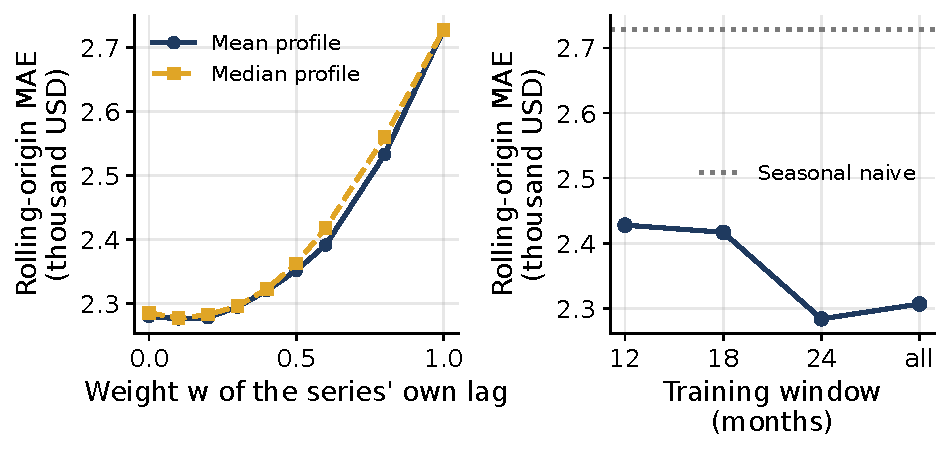
\includegraphics[width=\linewidth]{figures/sensitivity.pdf}
\caption{Izquierda: MAE de origen móvil del modelo propuesto con el peso $w$ fijo, para el perfil de medias y el de medianas; $w=1$ equivale al ingenuo estacional. Derecha: MAE de origen móvil según el máximo de meses de entrenamiento, con selección anidada de hiperparámetros; la línea punteada es el ingenuo estacional.}
\label{fig:sens}
\end{figure}

\subsection{Costo computacional}\label{subsec:costo}

La Tabla~\ref{tab:costo} reporta el costo. El modelo propuesto es el más rápido de ajustar (0.45 ms, unas 12 veces menos que Lasso, el más rápido de las referencias entrenadas, y unas 760 veces menos que Random Forest), el más rápido en inferencia (0.27 ms frente a 2.5--16 ms) y el más pequeño (0.35 kB). Dos precisiones: el ingenuo estacional no requiere ajuste alguno, de modo que la comparación de tiempos es entre modelos entrenados; y en la búsqueda completa de hiperparámetros Lasso es algo más rápido (0.09 s frente a 0.12 s), porque evalúa 4 configuraciones en paralelo frente a 12 en secuencia. En términos absolutos todos los tiempos son irrelevantes para una proyección mensual; lo relevante es que el modelo con menor error es también el más simple.

\begin{table}[!htb]
\caption{Costo computacional en la evaluación de origen móvil (mediana sobre los 24 orígenes). Búsqueda: tiempo total de la rejilla con validación cruzada. Ajuste e inferencia: reajuste de la configuración seleccionada y predicción de las 12 filas del mes, en un hilo. Tamaño: modelo serializado. Hardware: AMD Ryzen 5 7520U, 8 GB de RAM. En negrita el mejor valor de cada columna.}\label{tab:costo}
\footnotesize
\begin{tabular*}{\textwidth}{@{\extracolsep\fill}lrrrrr}
\toprule
Modelo & Config. & Búsqueda (s) & Ajuste (ms) & Inferencia (ms) & Tamaño (kB) \\
\midrule
Ridge & 5 & 0.13 & 5.6 & 2.7 & 2.3 \\
Lasso & 4 & \textbf{0.09} & 5.3 & 2.8 & 2.4 \\
Regresión bayesiana & 9 & 0.19 & 6.1 & 2.8 & 3.9 \\
KNN & 12 & 0.21 & 5.5 & 3.3 & 36.9 \\
Árbol de decisión & 16 & 0.28 & 5.5 & 2.5 & 3.3 \\
Random Forest & 24 & 10.35 & 344.6 & 16.0 & 858.7 \\
XGBoost & 24 & 1.99 & 62.7 & 3.7 & 309.1 \\
SVR & 18 & 0.39 & 9.9 & 3.1 & 25.3 \\
Modelo propuesto & 12 & 0.12 & \textbf{0.45} & \textbf{0.27} & \textbf{0.35} \\
\botrule
\end{tabular*}
\end{table}

\subsection{Interpretabilidad y análisis de errores}\label{subsec:errores}

\textbf{Interpretación.} El modelo es directamente legible: sus doce parámetros son el perfil de la Figura~\ref{fig:imp} (izquierda), estimado con 2015--2017. Enero y febrero venden 0.64 y 0.55 veces el promedio de los doce meses previos; marzo a agosto se mueven entre 0.80 y 1.14; septiembre (1.66), noviembre (1.94) y diciembre (1.75) son la temporada alta. El perfil coincide con la estacionalidad del análisis exploratorio y con lo esperable en el comercio minorista (cierre de año), y un planificador puede leerlo y discutirlo sin herramientas adicionales, lo que no ocurre con un ensamble de 300 árboles.

\begin{figure}[!htb]
\centering
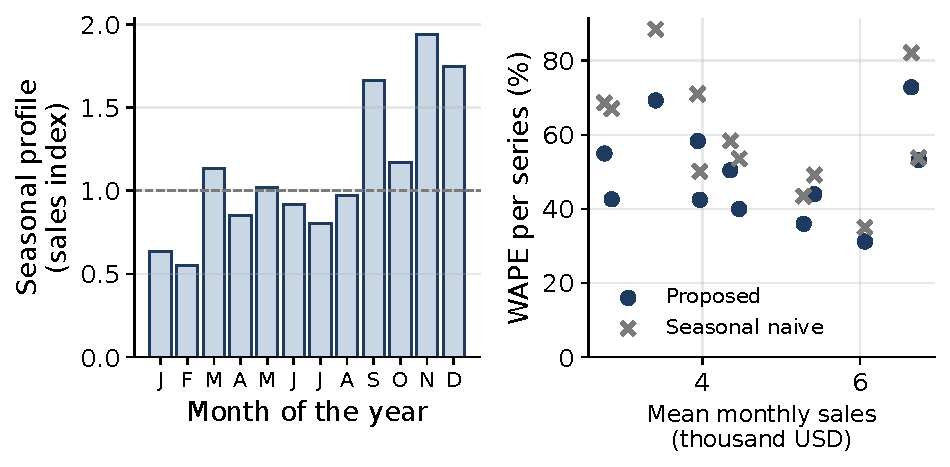
\includegraphics[width=\linewidth]{figures/profile_errors.pdf}
\caption{Izquierda: perfil estacional estimado con 2015--2017 (los doce parámetros del modelo); la línea discontinua es el nivel promedio de los doce meses previos. Derecha: WAPE por serie del modelo propuesto y del ingenuo estacional en la evaluación de origen móvil, frente a la venta mensual media de la serie.}
\label{fig:imp}
\end{figure}

\textbf{Errores por segmento.} El modelo mejora al ingenuo estacional en las 12 series y en 18 de los 24 meses (Figura~\ref{fig:imp}, derecha). El WAPE por serie va de 31.2\% (Muebles, Oeste) a 72.8\% (Tecnología, Este); las tres series con mayor error son de Tecnología (58.4--72.8\%), la categoría con más atípicos.

\textbf{Errores por rango del objetivo.} Al dividir las observaciones en terciles de venta aparece una regresión a la media: en el tercil bajo (venta media de 1{,}363 USD) el modelo sobrestima en promedio 1{,}323 USD y en el alto (8{,}867 USD) subestima 2{,}452 USD. En los tres terciles su MAE es menor que el del ingenuo estacional (1{,}430 frente a 1{,}588; 1{,}575 frente a 1{,}965; 3{,}915 frente a 4{,}630 USD). Los residuos tienen asimetría positiva (1.48): pocos errores grandes por subestimación (Figura~\ref{fig:pred}).

\textbf{Casos representativos.} Los cinco mayores errores son subestimaciones de picos, cuatro de ellos en Tecnología: Centro en octubre de 2016 (20{,}370 USD observados frente a 2{,}748 pronosticados), Este en octubre de 2017 y mayo de 2016, Oeste en marzo de 2017, y Oficina en el Centro en enero de 2017. Son meses dominados por pocos pedidos de alto valor, imprevisibles con un perfil estacional y con cualquiera de las variables disponibles. En el agregado, el modelo falla el cierre de 2017: subestima noviembre (118{,}448 USD observados frente a 107{,}478) y sobrestima diciembre (83{,}829 frente a 119{,}315), un mes que ese año cayó en lugar de ser el máximo (Figura~\ref{fig:serie}).

\subsection{Discusión, limitaciones y amenazas a la validez}\label{subsec:discusion}

\textbf{Discusión.} Tres resultados dialogan con la literatura. Primero, la agrupación de series es lo que hace funcionar al modelo, en línea con el principio de globalidad \cite{monteromanso2021}: lo que se comparte aquí no es un ensamble, sino doce números. Segundo, la ventaja de los ensambles de árboles reportada en competencias con miles de series \cite{makridakis2022} no se observa en un panel de 12 series y 36 meses: Random Forest es el mejor de los modelos generales en error cuadrático, pero no supera a un perfil estacional y cuesta cientos de veces más. La explicación más simple es de sesgo y varianza: con tan pocos datos, restringir el modelo a la estructura que el análisis exploratorio sugiere reduce más varianza de la que añade en sesgo. Tercero, el intercambio entre error absoluto y sesgo de nivel, visible en SVR, en la mediana y en el nivel estático, recuerda que el MAE premia pronósticos por debajo de la media cuando la distribución es asimétrica; para planificar totales, la métrica primaria debe leerse junto con el desvío del total.

\textbf{Aplicación.} Ese intercambio afecta directamente al uso del modelo. Al reentrenar con 2015--2017 para proyectar 2018, la validación cruzada elige por primera vez la mediana ($w=0$; MAE del índice de 0.560 frente a 0.573 del mejor perfil de medias), y la proyección anual resultante es de 653{,}057 USD, 10.9\% menos que las ventas de 2017. Con el perfil de medias ($w=0.1$) la proyección es de 866{,}415 USD, 18.2\% más. A la luz de la ablación, que mide un desvío de $-17.3$\% para la mediana frente a $-5.8$\% para la media, la segunda cifra es la adecuada para fijar metas e inventario; pero la discrepancia muestra que el criterio de selección por MAE no es neutral respecto del uso del pronóstico, y que la elección del estadístico debería fijarse según el objetivo de negocio y no dejarse a la validación cruzada.

\textbf{Limitaciones y amenazas a la validez.} (i) \emph{Diseño informado por los datos:} la idea del modelo surgió del análisis de un Random Forest evaluado sobre 2017, año que forma parte de la evaluación; 2016 no se usó como prueba en ese análisis y allí el margen es mayor, pero no puede descartarse un sesgo de selección a favor del modelo propuesto. (ii) \emph{Tamaño de muestra:} 24 bloques mensuales dan una potencia limitada, y la aproximación asintótica de las pruebas es frágil; la ausencia de significancia frente a siete referencias no demuestra equivalencia, ni su presencia frente a dos garantiza que se repita. (iii) \emph{Un solo conjunto de datos}, además de demostración: no se puede aplicar la prueba de Friedman ni afirmar generalización. El modelo supone una estacionalidad común a las series; donde no lo sea, la agrupación perjudicará. (iv) \emph{Primeros orígenes con poca historia:} con 12 a 17 meses, la validación interna tiene 2 o 3 pliegues y todos los modelos se ajustan con pocos datos, lo que favorece a los modelos simples. (v) \emph{Dependencia:} promediar por mes absorbe la correlación entre series, pero la prueba bayesiana supone una estructura de correlación solo aproximada. (vi) \emph{Variables:} no se usan promociones, precios ni calendario comercial, y el modelo solo produce pronósticos puntuales. (vii) \emph{Fuga de información:} todas las variables usan únicamente meses anteriores y toda estimación se hace dentro de la ventana de entrenamiento; no se identificó fuga más allá de lo señalado en (i). (viii) \emph{Tiempos:} las mediciones dependen del equipo y varían entre ejecuciones, aunque no el orden de magnitud.

\section{Conclusiones}\label{sec:conclusiones}

El objetivo se cumplió en la evaluación principal, con matices que deben quedar dichos. En 24 orígenes mensuales con reentrenamiento, el perfil estacional global obtuvo el menor error absoluto medio y el menor error cuadrático de los diez métodos, por debajo de Random Forest, XGBoost y SVR, y el menor tiempo de ajuste e inferencia entre los modelos entrenados, con doce parámetros que se leen directamente como la estacionalidad del negocio. La ventaja es estadísticamente concluyente frente al pronóstico ingenuo estacional, que representa la práctica actual, y frente a XGBoost; frente a Random Forest y al árbol de decisión hay indicios que no sobreviven a la corrección por comparaciones múltiples, y frente a SVR y KNN el modelo es equivalente en error. Los matices son tres: en la partición fija de 2017 SVR tuvo un error algo menor; el modelo no es el de menor desvío del total; y la búsqueda de hiperparámetros de Lasso es marginalmente más rápida. La ablación explica de dónde viene el resultado: lo decisivo es estimar la estacionalidad con todas las series agrupadas; el rezago de cada serie es prescindible, y el nivel móvil y la media no reducen el error por serie pero evitan subestimar el total entre una sexta y una cuarta parte.

Las limitaciones principales son que el diseño del modelo se benefició de un análisis previo sobre parte de los datos de evaluación, un único conjunto de datos de demostración, 24 meses que dejan poca potencia estadística, la ausencia de variables de promoción y precio, y pronósticos solo puntuales. Como trabajo futuro se propone: validar el modelo en conjuntos de datos no vistos durante su diseño y con más historia, para aplicar pruebas sobre varios conjuntos; simplificarlo fijando $w=0$ y la media; permitir perfiles parcialmente compartidos por categoría, contraídos hacia el común, cuando las series difieran en estacionalidad; elegir el estadístico del perfil con una pérdida acorde al uso del pronóstico y producir intervalos con perfiles cuantílicos; y reconciliar los pronósticos por serie con el total de la empresa.

\backmatter

\section*{Declaraciones}

\begin{itemize}
\item \textbf{Disponibilidad de datos:} Sample Superstore es un conjunto de datos público de demostración de Tableau Software \cite{superstore}. La copia utilizada (\texttt{data/raw/Sample - Superstore.csv}) y los datos procesados están en el repositorio del proyecto.
\item \textbf{Disponibilidad de código:} el código completo está en \url{https://github.com/AlexT09/SuperstorePython}. El ETL se ejecuta con \texttt{data/generate\_data.py}; el modelo propuesto está en \texttt{paper/perfil\_estacional.py} y todas las tablas, pruebas estadísticas y figuras de este artículo se reproducen con \texttt{paper/experimentos.py}. Las versiones de las librerías están en \texttt{requirements.txt} y la semilla aleatoria es 42. La aplicación interactiva (\url{https://superstorepython.onrender.com}) y el libro (\url{https://alext09.github.io/SuperstorePython/}) del proyecto corresponden a la primera versión del estudio y usan Random Forest.
\item \textbf{Contribución de los autores:} ambos autores participaron en el diseño del estudio, la implementación, el análisis de resultados y la redacción, y aprobaron la versión final.
\item \textbf{Conflicto de intereses:} los autores declaran no tener conflictos de interés.
\end{itemize}

\bibliography{sn-bibliography}

\end{document}
